\documentclass[12pt]{article}
\usepackage{amsmath,amssymb,amsfonts,amsthm}
\usepackage{geometry}
\usepackage{setspace}      % For double spacing
% \usepackage{mathptmx}      % Times New Roman font
\usepackage{physics}
\usepackage[hidelinks]{hyperref}
\usepackage{color}
\usepackage{xcolor}
\usepackage{subcaption}
\usepackage{tikz}
\usepackage{tikz-3dplot}
\usetikzlibrary{backgrounds, intersections}
\usetikzlibrary{calc}
\usetikzlibrary{math}
\usetikzlibrary{shapes.geometric}
\usepackage{pgfplots}
\usepackage{enumitem}
\usepackage{xcolor}
\usepackage[english]{babel}
\usepackage[autostyle]{csquotes}

\pgfplotsset{compat=1.18}

\geometry{margin=1in}

% Set double spacing
\setstretch{1.5}

\newcommand{\todo}[1]{\textcolor{red}{#1}}
\newcommand{\note}[1]{\textcolor{blue}{#1}}

\newcommand{\R}{\mathbb{R}}
\newcommand{\C}{\mathbb{C}}
\newcommand{\Z}{\mathbb{Z}}
\newcommand{\N}{\mathbb{N}}
\newcommand{\Q}{\mathbb{Q}}
\newcommand{\F}{\mathbb{F}}


\tdplotsetmaincoords{60}{130}     % your camera
\tdplotsetrotatedcoords{35}{-45}{0}  % so that the plane is z'=0


\newtheorem{definition}{Definition}[section]
\newtheorem{theorem}[definition]{Theorem}
\newtheorem{proposition}[definition]{Proposition}
\newtheorem{corollary}[definition]{Corollary}

\geometry{margin=1in}
\title{A look at Geodesics through the lens of symmetries and its applications to Black Holes}
\author{Ulizes Raudales}
\date{\today}

\begin{document}
\maketitle

\newpage
\tableofcontents
\newpage

\begin{abstract}
	This thesis presents a coherent framework for the analysis of geodesics both on smooth two-dimensional surfaces in \(\R^3\) and in the Schwarzschild spacetime of a black hole.
	Beginning with the derivation of the geodesic equations, we show how continuous isometries give rise to first integrals via Killing vector fields.  
	Specializing to surfaces of revolution, we recover Clairaut's relation and illustrate its use on different surfaces, including the torus and the hyperboloid
	We then apply the same symmetry-based methods to the Schwarzschild metric, deriving the effective potential for null and time-like geodesics, locating circular orbits, and identifying the photon sphere.  
	Throughout, the unified emphasis on symmetry yields both conceptual clarity and practical computational shortcuts.
\end{abstract}

\section{Introduction}

In many applications—ranging from navigation on the Earth’s surface to path planning in computer graphics and robotics—we seek the “straightest” or shortest route between two points on a curved surface.  
In the flat plane, these are ordinary straight lines; on a curved surface, they become \emph{geodesics}, which locally minimize distance while remaining intrinsic to the surface.

Finding geodesics by solving the full system of second‐order differential equations can be algebraically intensive.  
However, when a surface admits continuous symmetries, one can exploit those isometries to obtain conserved quantities that greatly simplify the problem.  
In this thesis, we develop a unified, symmetry‐based approach to geodesic analysis.

After reviewing the necessary tools from differential geometry (Section 1), we derive the general geodesic equations on an arbitrary surface (Section 2).  
Section 3 specializes to surfaces of revolution, where Clairaut’s relation emerges as a consequence of rotational symmetry.  
In Section 4, we introduce Killing vector fields and Noether’s theorem to explain how each continuous symmetry produces a conserved quantity.  
Finally, in Section 5, we apply these methods to the Schwarzschild spacetime—deriving the effective potential for time‐like and null geodesics, locating circular orbits, and characterizing the photon sphere.

\section{Background and Preliminaries}

Differential geometry combines the tools of calculus and algebra to study geometric structures, with applications in physics, engineering, and computer science. 
In this section, we introduce the basic concepts and tools that will appear throughout this thesis.

\medskip
\noindent
First, we define the central object of study.

\begin{definition}[Manifold]\label{def:manifold}
A \emph{manifold} $M$ is a smooth $n$-dimensional topological space that locally ressembles $\mathbb{R}^n$.
\end{definition}

Intuitively, manifolds generalize curves and surfaces to arbitrary dimensions. They possess several key features:
\begin{itemize}
  \item \textbf{Metric Spaces: } Manifolds are smoothly varying metric spaces, meaning they have a well-defined notion of distance and angle.
  \item \textbf{Differentiable Structure.} Manifolds have a differentiable structure, allowing us to define smooth functions, tangent vectors, and derivatives.
\end{itemize}

\medskip
\noindent
Next, we introduce the mappings that preserve the manifold structure.

\begin{definition}[Diffeomorphism]\label{def:diffeomorphism}
A map $\varphi\colon M \to N$ between smooth manifolds is a \emph{diffeomorphism} if it is bijective, smooth, and its inverse $\varphi^{-1}$ is also smooth. 
If such a map exists, $M$ and $N$ are said to be \emph{diffeomorphic}. 
A diffeomorphism from $M$ to itself is called a \emph{self‑diffeomorphism}.
\end{definition}

\medskip
\noindent
Finally, we remark on \emph{tensors}, mathematical objects that generalize vectors and matrices to arbitrary dimensions and are used to describe geometric and physical quantities in a coordinate-independent manner.
Although tensors are fundamental in differential geometry, their full development lies beyond the scope of this thesis, so we will introduce them only when needed.

A quick note on notation: 
\begin{itemize}
	\item We use latin letter subscripts to denote derivatives with respect to the corresponding coordinate.
	\item We use Newton's notation for derivatives with respect to time, i.e., $\dot{q} = \frac{dq}{dt}$.
	\item We use greek letters to denote the coordinates of the manifold and for the components of tensors.
	\item Is convention to use the Einstein summation convention, where repeated indices are summed over. However, we will not use this convention in this thesis to avoid confusion.
\end{itemize}

\subsection{Surfaces in \texorpdfstring{$\mathbb{R}^3$}{R3}}\label{sec:surface-def}

We will focus on \emph{surfaces}, which are 2-dimensional manifolds embedded, i.e., smoothly and continuously mapped, in $\mathbb{R}^3$.
The embedding in $\mathbb{R}^3$ endows the surface with additional geometric structure (coming from the ambient Euclidean geometry) that allows us to measure distances, angles, and curvature.

\begin{definition}[Surface]\label{def:surface}
	A regular surface $\mathcal{S}\subset\R^3$ is the image of a one-to-one smooth map that maps an open set $U\subset\R^{2}$ into $\R^3$:
	\begin{equation}\label{eq:surface-param}		
		\mathbf{r}: U\subset\R^{2}\to\R^3 \qquad \mathbf{r}(u,v) = \begin{bmatrix}
			x(u,v)\\[1ex]
			y(u,v)\\[1ex]
			z(u,v)
		\end{bmatrix}
	\end{equation}
	with $\mathbf{r}$ being regular(i.e., $\pdv{\mathbf{r}}{u} \times \pdv{\mathbf{r}}{v} \neq 0$ for all $(u,v)\in U$).
\end{definition}

For clarity, denote the surface by $\mathcal{S}=\mathbf{r}(U)$. At any point $\mathbf{r}(u_0,v_0)$, the tangent vectors are given by
\[
\mathbf{r}_u = \pdv{\mathbf{r}}{u}, \quad \mathbf{r}_v = \pdv{\mathbf{r}}{v},
\]
which span the tangent plane at some point $p = \mathbf{r}(u_0,v_0)$, that is 
\[
T_{p}(\mathcal{S}) = \text{span}\{\mathbf{r}_u,\mathbf{r}_v\}.
\]
where $T_{p}(\mathcal{S})$ is the tangent space at point $p$.
So by definition, for any tanget vector $\mathbf{v}\in T_{p}(\mathcal{S})$, we can write
\[
\mathbf{v} = a\mathbf{r}_u + b\mathbf{r}_v,
\]
where $a,b\in\R$ are real numbers.

We have that the unit normal vector $\mathbf{U}$ to the surface at point $p$ is given by
\[
\mathbf{U} = \frac{\mathbf{r}_u\times\mathbf{r}_v}{\|\mathbf{r}_u\times\mathbf{r}_v\|}.
\]
which is a unit vector orthogonal to the tangent plane at point $p$.

\subsection{The Metric on a Surface}
The \emph{metric}, which is a smoothly varying inner product on the tangent plane at each point allows us to measure lengths of curves, angles between tangent vectors, and surface areas. 
For an embedded surface with local coordinates $(u,v)$, the metric (also called the \emph{first fundamental form}) can be obtained by restricting the Euclidean dot product to the tangent plane:
\[
g_{\,\mu\nu} = \mathbf{r}_\mu\,\cdot\,\mathbf{r}_\nu, \qquad \mu,\nu \in \{u,v\}.
\]
In matrix form, the metric tensor can be written as 
\[
g_{\mu\nu} = 
\begin{bmatrix}
E & F\\[1ex]
F & G
\end{bmatrix},
\] 
where 
\begin{equation}\label{eq:metric-coefficients}
	E = \mathbf{r}_u\cdot \mathbf{r}_u, \qquad F = \mathbf{r}_u\cdot \mathbf{r}_v, \qquad G = \mathbf{r}_v\cdot \mathbf{r}_v.
\end{equation}

Thus, for an infinitesimal displacement $dq = (du,\;dv)^\top$ in the parameter domain, the squared distance traveled on the surface is 
\begin{equation}\label{eq:line-element}
ds^{2} \;=\; \begin{bmatrix}
	E & F\\[1ex]
	F & G
\end{bmatrix} \begin{bmatrix}
	du\\[1ex]
	dv
\end{bmatrix} \begin{bmatrix}
	du\\[1ex]
	dv
\end{bmatrix}^{\top} \;=\; E\,du^{2} + 2F\,du\,dv + G\,dv^{2}.
\end{equation}
This is the \emph{line element} of the surface, which describes how distances are measured on the surface.

We find the length of the line element by the following:
\[
	L = \int_{a}^{b} \sqrt{ds^{2}} \, dt
\]

\subsection{Curves on a Surface}
With the metric in hand, we can consider curves drawn on the surface and measure their lengths. 

\begin{definition}[Curve on a Surface]\label{def:curve}
A (parametrized) curve $\gamma$ on a surface $\mathcal{S}$ is a smooth map $\gamma: I \to \mathcal{S}$ from an interval $I\subset \mathbb{R}$ into the surface. 
Writing 
\begin{equation}\label{eq:curve-param}
	\gamma(t) = \mathbf{r}(u(t), v(t))
\end{equation}
in terms of a local parametrization of $\mathcal{S}$, the coordinates $(u(t), v(t))$ describe the path of the curve in the parameter domain. 
\end{definition}
The velocity (tangent) vector of $\gamma$ at parameter $t$ is 
\begin{equation}\label{eq:curve-vel}
	\dot\gamma(t) = \frac{d}{dt}\mathbf{r}(u(t), v(t)) = \dot{u}(t)\,\mathbf{r}_u + \dot{v}(t)\,\mathbf{r}_v,
\end{equation}
which indeed lies in the tangent plane $T_{\gamma(t)}(\mathcal{S})$. 


\begin{definition}[Unit Speed Curve]\label{def:unit-speed}
A curve $\gamma(t)$ on $\mathcal{S}$ is \emph{unit speed} (or parametrized by arc length) if the following condition holds for all $t$:
\[
\|\dot{\gamma}(t)\|^{2} = 1
\] 
\end{definition}

Under this condition, the parameter $t$ itself represents the arc length along the curve. 


\subsection{Arc Length Reparametrization}
Any regular curve $\gamma(t)$ can be reparametrized to have unit speed (except at points where $\dot\gamma=0$). 
This is done by defining a new parameter $s$ as the arc length from some fixed point $t_0$ to $t$:
\[
s(t) = \int_{t_0}^{t} \|\dot\gamma(t)\|\,dt 
\]
By the Fundamental Theorem of Calculus, we have that $\dot{s}(t) = \|\dot\gamma(t)\| > 0$.
By the Mean Value Theorem, $s(t)$ is a strictly increasing function of $t$ and thus has an inverse function $t(s)$.
Now define a new curve \(\beta(s)\) by reparameterizing \(\gamma(t)\) with respect to the arc length \(s\):
\[
\beta(s)=\gamma(t(s)).
\]
We can show that \(\beta(s)\) is a unit speed curve.
By the chain rule,
\[
\dv{s}\beta(s) = \frac{d}{ds}\gamma(t(s)) = \gamma'(t(s))\,\frac{dt}{ds}.
\]
where 
\[
\frac{dt}{ds} = \frac{1}{\|\gamma'(t(s))\|}.
\]
Substitute the expression for \(\frac{dt}{ds}\) into the derivative of \(\beta(s)\),
\[
\dv{s}\beta(s) = \gamma'(t(s))\cdot \frac{1}{\|\gamma'(t(s))\|}.
\]
Taking the norm of both sides,
\[
\left\|\dv{s}\beta(s)\right\| = \left\|\gamma'(t(s)) \cdot \frac{1}{\|\gamma'(t(s))\|}\right\| = \frac{\|\gamma'(t(s))\|}{\|\gamma'(t(s))\|} = 1.
\]
Therefore, all curves can be reparameterized to have unit speed.

Under arc length reparametrization, we call $s$ the \emph{arc length parameter} or \emph{proper time} in the context of general relativity.
This parameter is usually refered as the \emph{affine parameter} in the context of geodesics, as it is a parameter that preserves the affine structure of the curve.
Affine parameters are exactly those parameters for which the geodesic equation has no extra “forcing” term.

\subsection{Curvature}
The curvature of a curve is a measure of how much the curve deviates from being a straight line.
In Euclidean space, the curvature of a curve is defined as the rate of change of the tangent vector with respect to the arc length parameter.

\begin{definition}[Curvature]\label{def:curvature}
	The curvature of a curve $\gamma(t)$ is defined as
	\[
	\kappa_{\gamma} = \frac{\|\dot{\gamma}\times\ddot{\gamma}\|}{\|\dot{\gamma}\|^{3}}.
	\]
	For a unit speed curve, this simplifies to
	\[
	\kappa_{\beta}(s) = \|\ddot{\beta}(s)\|.
	\]
\end{definition}
The curvature is a scalar quantity that describes how much the curve bends at a given point.

Another important quantity related to curvature is the normal curvature, which is the projecction of the curvature vector onto the normal vector of the surface at that point.
\[
	\kappa_{\mathbf{N}} = \mathbf{N} \cdot \kappa_{\gamma}
\]
The normal curvature is a measure of how much the curve bends in the direction of the normal vector at that point.


\section{Geodesics}
% When working on surfaces, we want to find the \enquote{straightest} paths between two points on the surface, which are usually the shortest paths.
% In Euclidean space, the straightest path between two points is a straight line.
% However, on a curved surface, the shortest path may not be a straight line in the Euclidean sense.

Another important quantity related to curvature is the \emph{geodesic curvature}, which is how much the curve deviates from being a geodesic on the surface.
Which is defined as 
\begin{equation}\label{eq:geodesic-curvature}
	\kappa_{g} = \kappa_{\gamma} - \kappa_{\mathbf{N}}.
\end{equation}

This provides a measure of how much the curve deviates from being a straight line on the surface.

\begin{definition}[Geodesic]\label{def:geodesic}
	A curve $\gamma(t)$ on a surface $\mathcal{S}$ or any manifold $\mathcal{M}$ is called a \emph{geodesic} if it is the \enquote{straightest} path between two points on the surface.
	More formally, a curve is a geodesic if it has zero geodesic curvature:
	\[
		\kappa_{g} = 0.
	\]
\end{definition}
Intuitively, one can think of a geodesic as a path for which one can travel in a straight line without having to turn or change direction.
Essentially, a geodesic is a curve that is "straight" in the sense that it does not curve away from the surface.

A geodesic can also be thought as the shortest path between two points on a surface.
However, this is not always the case, as shown in \cite{jia2024geodesics} and will be discussed in more detail once we explore geodesics on different surfaces.

\subsection{Deriving the Geodesic Equation}

To find the geodesics of a surface, we let $\gamma(t)$ be a geodesic on a surface $\mathcal{S}$; the curve parameterized in terms of Eq.(\ref{eq:curve-param}) and find its velocity vector Eq.(\ref{eq:curve-vel}).
We can also find the acceleration vector of the curve by differentiating the velocity vector with respect to $t$:
\begin{equation}\label{eq:curve-acc}
	\ddot\gamma(t) = \dot{u}(t)^{2}\mathbf{r}_{uu} + \dot{v}(t)^{2}\mathbf{r}_{vv} + 2\dot{u}(t)\dot{v}(t)\mathbf{r}_{uv} + \ddot{u}\mathbf{r}_{u} + \ddot{v}\mathbf{r}_{v}.
\end{equation}

We can break $\ddot{\gamma}(t)$ into two components: the tangential component to the surface and the normal component to the surface.
\begin{equation}\label{eq:curve-acc-decomp}
	\ddot{\gamma}(t) = \ddot{\gamma}_{\text{norm}}(t) + \ddot{\gamma}_{\text{tan}}(t),
\end{equation}

The normal component, $\ddot{\gamma}_{\text{norm}}(t)$, is the curvature imposed by the surface on the curve, while the tangential component, $\ddot{\gamma}_{\text{tan}}(t)$, is any extra curvature imposed by the curve itself.
We thus have
\[
	\kappa_{g} = \ddot{\gamma}_{\text{tan}}(t) \cdot \mathbf{U} = 0,
\]
The derivation for rhe tangential component of the acceleration vector is outside the scope of this thesis, but its derivation can be found in \cite{celano2022why}\cite{oprea2007differential}, so we have 
\[
	\ddot{\gamma}_{\text{tan}}(t) = \ddot{\gamma} \cdot \mathbf{r}_{u} + \ddot{\gamma} \cdot \mathbf{r}_{v} = 0.
\]
Since we want the geodesic curvature to be zero, and since both components are linearly independent, the dot products cannot be additive inverses of each other, so we can set them to zero:
\[
	\ddot{\gamma}(t) \cdot \mathbf{r}_{u} = 0, \qquad \ddot{\gamma}(t) \cdot \mathbf{r}_{v} = 0.
\]	
Substituting the expression for $\ddot{\gamma}(t)$ from Eq.(\ref{eq:curve-acc}) into these two equations gives us two second-order ordinary differential equations for $u(t)$ and $v(t)$:
\begin{align*}
	\ddot{\gamma} \cdot \mathbf{r}_{u} = \dot{u}(t)^{2}\mathbf{r}_{uu} \cdot \mathbf{r}_{u} + \dot{v}(t)^{2}\mathbf{r}_{vv} \cdot \mathbf{r}_{u} + 2\dot{u}(t)\dot{v}(t)\mathbf{r}_{uv} \cdot \mathbf{r}_{u} + \ddot{u}\mathbf{r}_{u} \cdot \mathbf{r}_{u} + \ddot{v}\mathbf{r}_{v} \cdot \mathbf{r}_{u} = 0 \\
	\ddot{\gamma} \cdot \mathbf{r}_{v} = \dot{u}(t)^{2}\mathbf{r}_{uu} \cdot \mathbf{r}_{v} + \dot{v}(t)^{2}\mathbf{r}_{vv} \cdot \mathbf{r}_{v} + 2\dot{u}(t)\dot{v}(t)\mathbf{r}_{uv} \cdot \mathbf{r}_{v} + \ddot{u}\mathbf{r}_{u} \cdot \mathbf{r}_{v} + \ddot{v}\mathbf{r}_{v} \cdot \mathbf{r}_{v} = 0. 
\end{align*}
Because $\mathbf{r}_{u}$ and $\mathbf{r}_{v}$ are orthogonal and thus $\mathbf{r}_{u}\cdot\mathbf{r}_{v} = 0$, and isolating the second derivatives gives us the following two equations:
\begin{align}
	\ddot{u} + \dot{u}(t)^{2}\frac{\mathbf{r}_{uu} \cdot \mathbf{r}_{u}}{\mathbf{r}_{u} \cdot \mathbf{r}_{u}} + \dot{v}(t)^{2}\frac{\mathbf{r}_{vv} \cdot \mathbf{r}_{u}}{\mathbf{r}_{u} \cdot \mathbf{r}_{u}} + 2\dot{u}(t)\dot{v}(t)\frac{\mathbf{r}_{uv} \cdot \mathbf{r}_{u}}{\mathbf{r}_{u} \cdot \mathbf{r}_{u}} = 0 \label{eq:geodesic-acc-decomp-1}\\
	\ddot{v} + \dot{u}(t)^{2}\frac{\mathbf{r}_{uu} \cdot \mathbf{r}_{v}}{\mathbf{r}_{v} \cdot \mathbf{r}_{v}} + \dot{v}(t)^{2}\frac{\mathbf{r}_{vv} \cdot \mathbf{r}_{v}}{\mathbf{r}_{v} \cdot \mathbf{r}_{v}} + 2\dot{u}(t)\dot{v}(t)\frac{\mathbf{r}_{uv} \cdot \mathbf{r}_{v}}{\mathbf{r}_{v} \cdot \mathbf{r}_{v}} = 0. \label{eq:geodesic-acc-decomp-2}
\end{align}
Recall that by Eq.(\ref{eq:metric-coefficients}), we have
\[
	E = \mathbf{r}_{u} \cdot \mathbf{r}_{u}  \qquad F = \mathbf{r}_{u} \cdot \mathbf{r}_{v} \qquad G = \mathbf{r}_{v} \cdot \mathbf{r}_{v}\\
\]
Taking the derivatives of each coefficient with respect to $u$ and $v$ gives us the following relationships:
\begin{alignat*}{4}
E_{u} \; &=\; 2\,\mathbf{r}_{uu}\cdot \mathbf{r}_{u} \quad &\quad E_{v} \; &=\; 2\,\mathbf{r}_{uv}\cdot \mathbf{r}_{u}\\[5pt]
F_{u} \; &=\; \mathbf{r}_{uu}\cdot \mathbf{r}_{v} + \mathbf{r}_{u}\cdot \mathbf{r}_{uv} \quad &\quad F_{v} \; &=\; \mathbf{r}_{uv}\cdot \mathbf{r}_{v} + \mathbf{r}_{u}\cdot \mathbf{r}_{vv}\\[5pt]
G_{u} \; &=\; 2\,\mathbf{r}_{vu}\cdot \mathbf{r}_{v} \quad &\quad G_{v} \; &=\; 2\,\mathbf{r}_{vv}\cdot \mathbf{r}_{v}
\end{alignat*}
Substituting these relationships into the equations (\ref{eq:geodesic-acc-decomp-1}) and (\ref{eq:geodesic-acc-decomp-2}) gives us the following two equations:
\begin{equation}\label{eq:geodesic-uv}
	\ddot{u} + \frac{E_{u}}{2E}\dot{u}^{2} + \frac{E_{v}}{E}\dot{u}\dot{v} - \frac{G_{u}}{2E}\dot{v}^{2} = 0
\end{equation}
\begin{equation}\label{eq:geodesic-vu}
	\ddot{v} - \frac{E_{v}}{2G}\dot{u}^{2} + \frac{G_{u}}{G}\dot{u}\dot{v} + \frac{G_{v}}{2G}\dot{v}^{2} = 0
\end{equation}

These two equations are the geodesic equations for the coordinates \(u\) and \(v\) on the surface.
These equations correspond to the case where $F = 0$, as the equations are independent of the cross term $F$.
For our look at surfaces of revolution, we have that $F = 0$, as the surface is symmetric about the axis of rotation.


In the case where $F \neq 0$, we can write the geodesic equations in a more general form:
\begin{equation}\label{eq:geodesic-compact}
	\dv[2]{q^\sigma}{t} + \sum_{\mu,\nu=1}^{n} \Gamma_{\mu\nu}^\sigma \dv{q^\mu}{t} \dv{q^\nu}{t} = 0,
\end{equation}
where $n$ is the number of coordinates on the surface, and $q^\sigma$ are the coordinates on the surface.
$\Gamma_{\mu\nu}^\sigma$ are the \emph{Christoffel symbols} of the second kind, which describe how the metric changes as we move along the surface.
The \emph{Christoffel symbols} are defined as:
\[
	\Gamma_{\mu\nu}^\sigma = \frac{1}{2}\sum_{\lambda=1}^{n}g^{\sigma\lambda}\left(\pdv{g_{\mu\nu}}{q^\lambda} + \pdv{g_{\nu\lambda}}{q^\mu} - \pdv{g_{\mu\lambda}}{q^\nu}\right)
\]
It tells us how much the rate of change in the $\mu$-th coordinate depends on the $\nu$-th coordinate as we move along the $\sigma$-th coordinate.
On Surfaces, the Christoffel symbols can be computed to be:
\[
\begin{aligned}
	\Gamma_{uu}^{u} &= \frac{1}{2(EG - F^{2})}\bigg[ G E_{u} - F (2F_{u} + E_{v}) \bigg] &\qquad \Gamma_{uv}^{u} &= \Gamma_{vu}^{u} = \frac{1}{2(EG - F^{2})}\bigg[ G E_{v} - F G_{u} \bigg] \\
	\Gamma_{vv}^{u} &= \frac{1}{2(EG - F^{2})}\bigg[ G (2F_{v} - G_{u}) - F G_{v} \bigg] &\qquad \Gamma_{uu}^{v} &= \frac{1}{2(EG - F^{2})}\bigg[ E (2F_{u} - E_{v}) - F E_{u} \bigg] \\
	\Gamma_{uv}^{v} &= \Gamma_{vu}^{v} = \frac{1}{2(EG - F^{2})}\bigg[ E G_{u} - F E_{v} \bigg] &\qquad \Gamma_{vv}^{v} &= \frac{1}{2(EG - F^{2})}\bigg[ E G_{v} - F (2F_{v} + G_{u}) \bigg] \\
\end{aligned}
\]
The geodesic equations for a surface $\mathcal{S}$ are given by:
\[
	\ddot{u} + \Gamma_{uu}^{u}\dot{u}^{2} + 2\Gamma_{uv}^{u}\dot{u}\dot{v} + \Gamma_{vv}^{u}\dot{v}^{2} = 0
\]
\[
	\ddot{v} + \Gamma_{uu}^{v}\dot{u}^{2} + 2\Gamma_{uv}^{v}\dot{u}\dot{v} + \Gamma_{vv}^{v}\dot{v}^{2} = 0
\]
In our case of equations (\ref{eq:geodesic-uv}) and (\ref{eq:geodesic-vu}), we have $F = 0$, so the Christoffel symbols simplify to:
\[
\begin{aligned}
    \Gamma_{11}^{1} &= \frac{E_{u}}{2E} &\quad \Gamma_{12}^{1} &= \Gamma_{21}^{1} = \frac{E_{v}}{2E} &\quad \Gamma_{22}^{1} &= -\frac{G_{u}}{2E} \\[4mm]
    \Gamma_{11}^{2} &= -\frac{E_{v}}{2G} &\quad \Gamma_{12}^{2} &= \Gamma_{21}^{2} = \frac{G_{u}}{2G} &\quad \Gamma_{22}^{2} &= -\frac{G_{v}}{2G}.
\end{aligned}
\]

\section{Geodesics on Surfaces of Revolution}

Surfaces of revolution are a class of surfaces obtained by rotating a planar curve about an axis in the plane. 
They are highly symmetric surfaces, exhibiting rotational symmetry.

\begin{figure}[ht]
	\centering
	\begin{minipage}{0.48\textwidth}
	    \centering
		\begin{tikzpicture}[scale=1.2]
			\tikzmath{function f(\t) {return 1.5 + 0.35*sin(\t r);};}
			% Axes in the xz-plane
			\draw[->] (-2,0) -- (2,0) node[right] {$x$};
			\draw[->] (0,-2) -- (0,2) node[above] {$z$};
			\draw[dashed] (0,1) -- (1.8,1) node[midway, above] {$x(u)$};
			\draw[dashed] (1.8,0) -- (1.8,1) node[midway, right] {$z(u)$};

			% Plot of the profile curve: x = f(t), z = t
			\draw[domain=-2:2, smooth, variable=\t, red, ultra thick] plot ({f(\t)},{\t});
			\node at (2.5,2) {$\gamma(t)$};
		\end{tikzpicture}
		\subcaption{2D profile in the $xz$-plane}
	\end{minipage}
	\hfill
	\begin{minipage}{0.48\textwidth}
	    \centering
		\tdplotsetmaincoords{60}{130}
		\begin{tikzpicture}[tdplot_main_coords]
			% The function that is rotated
			\tikzmath{function f(\x) {return 1.5 + 0.35*sin(\x r);};}
			\pgfmathsetmacro{\dominio}{2.0}
			\pgfmathsetmacro{\xi}{-\dominio}
			\pgfmathsetmacro{\step}{(\dominio-\xi)/70.0}
			\pgfmathsetmacro{\xs}{\xi+\step}
			\pgfmathsetmacro{\max}{3}
			% Circumferences (behind the coordinate axis)
			\foreach \z in {\xi,\xs,...,\dominio}{
				\pgfmathsetmacro{\radio}{f(\z)}
				\draw[cyan,very thick,opacity=0.35] plot[domain=0:2.0*pi,smooth,variable=\t] ({\radio*cos(\t r)},{\radio*sin(\t r)},{\z});
			}
			% Graph of the function rotated about the $y$ axis
			\draw[red,ultra thick] plot[domain=-\dominio:\dominio,smooth,variable=\t] ({f(\t)},{0},{\t}) node [right, sloped] {$z = \gamma(t)$};
			% Coordinate axis
			\draw[thick,->] (0,0,0) -- (0,\max,0) node [right] {$y$};
			\draw[thick,->] (0,0,0) -- (0,-\max,0) node [above] {$-y$};
			\draw[thick,->] (0,0,0) -- (\max,0,0) node [left] {$x$};
			\draw[thick,->] (0,0,0) -- (-\max,0,0) node [below] {$-x$};
			\draw[thick,->] (0,0,0) -- (0,0,\max) node [above] {$z$};
			% Draw a grid in the xy-plane at z=0
			\begin{scope}[canvas is xy plane at z=0]
				\draw[gray, step=0.5cm, opacity=0.25] (-\max,-\max) grid (\max,\max);
			\end{scope}
		\end{tikzpicture}
		\subcaption{3D view of $\gamma(t)$}
	\end{minipage}

	\caption{Profile Curve and Corresponding Surface of Revolution}
\end{figure}

\begin{definition}[Surface of Revolution]\label{def:surf-rev}
A surface of revolution is a surface obtained by rotating a $C^{2}$-smooth plane curve $\gamma(u) = (f(u), g(u))$ about an axis in the plane. 
The curve $\gamma(u)$ is called the \emph{profile curve} of the surface. 
\end{definition}
We will focus on surfaces of revolution generated by rotation about the $z$-axis.
Thus our profile curve $\gamma(u)$ lies in the $xz$-plane, and we can write it as $\gamma(u) = (x(u), z(u))$ with $x(u)\ge 0$.

A convenient parametrization for this surface is:
\begin{equation}\label{eq:param-rev}
\mathbf{r}(u,v) = \begin{bmatrix}
x(u)\cos v\\[1ex]
x(u)\sin v\\[1ex]
z(u)
\end{bmatrix}, 
\end{equation}
where $u$ runs along the profile curve and $v$ is the rotation angle about the $z$-axis. 
Here $0 \le v < 2\pi$ and $u$ is in some interval $I$ corresponding to the domain of the profile curve. 
In this parametrization, $u$ is the coordinate along the meridian (profile curve) and $v$ is the angular coordinate (longitude).

Let us derive the metric for a surface of revolution given by \eqref{eq:param-rev}. 
First, the partial derivatives of $\mathbf{r}(u,v)$ are:
\[
\mathbf{r}_u = \begin{bmatrix} x_{u}\cos v \\ x_{u}\sin v \\ z_{u} \end{bmatrix}, \qquad 
\mathbf{r}_v = \begin{bmatrix} -\,x(u)\sin v \\ \phantom{-}x(u)\cos v \\ 0 \end{bmatrix}.
\]
The dot products yield the metric components:
\[
E = \mathbf{r}_u \cdot \mathbf{r}_u = x_{u}^{2} + z_{u}^{2}, \qquad 
F = \mathbf{r}_u \cdot \mathbf{r}_v = 0, \qquad 
G = \mathbf{r}_v \cdot \mathbf{r}_v = [\,x(u)\,]^{2}.
\]
We see that $F=0$ for this standard parametrization of a surface of revolution, which means the coordinate lines $u=\text{const}$ (circles of latitude) and $v=\text{const}$ (meridians) meet orthogonally on the surface. 

Thus, the first fundamental form is
\begin{equation}\label{eq:metric-rev}
ds^{2} \;=\; \big(x_{u}^{2} + z_{u}^{2}\big)\,du^{2} + x(u)^{2}\,dv^{2}\,.
\end{equation}
This succinctly captures the geometry: $x(u)$ acts as the “radius” of the parallel (circle of latitude) at that $u$-value, and $\sqrt{x_{u}^{2}+z_{u}^{2}}\,du$ is the element of arc length along the meridian.

Taking the derivatives of the components of the metric, we find:	
\[
E_{u} = 2(x_{u}x_{uu} + z_{u}z_{uu}), \quad E_{v} = 0, \quad G_{u} = 2xx_{u}, \quad G_{v} = 0.
\]
Thus, the geodesic equations for a surface of revolution reduce to
\begin{align}
	\ddot{u} + \frac{x_{u}x_{uu} + z_{u}z_{uu}}{x_{u}^{2} + z_{u}^{2}}\,\dot{u}^2 - \frac{x x_{u}}{x_{u}^{2} + z_{u}^{2}}\,\dot{v}^{2} &= 0 \label{eq:geodesic-u}\\
	\ddot{v} - 2\frac{x_{u}}{x}\dot{u}\dot{v} &= 0 \label{eq:geodesic-v}
\end{align}

Under arc length parametrization, we have the following:
\[
	x_{u}^{2} + z_{u}^{2} = 1 \qquad 2(x_{u}x_{uu} + z_{u}z_{uu}) = 0 
\]

Thus, the geodesic equations reduce to
\begin{align}
	\ddot{u} - x x_{u}\,\dot{v}^{2} &= 0 \label{eq:geodesic-u-arc}\\
	\ddot{v} - 2\frac{x_{u}}{x}\dot{u}\dot{v} &= 0 \label{eq:geodesic-v-arc}
\end{align}

Looking at the metric for a unit speed curve, we have
\[
	ds^{2} = du^{2} + x(u)^{2}dv^{2} 
\]
We then have the following must hold for a unit speed curve:
\begin{equation}\label{eq:unit-speed-condition}
	1 = \left(\dv{u}{s}\right)^{2} + x(u)^{2}\left(\dv{v}{s}\right)^{2} 
\end{equation}
This means that the geodesic equations are not independent of the unit speed condition, and thus we must solve them simultaneously.

\subsection{Meridian and Parallel Geodesics}
We can extrapolate some general geodesics in surfaces of revolution by keeping one of the coordinates constant.
With this, we will find two types of geodesics: the \emph{meridian geodesic} and the \emph{parallel geodesic}.

Meridian geodesics are geodesics that run along the longitude (top to bottom) of the surface.
To find the meridian geodesics, we set $v = \text{const}$, which means $\dot{v} = \ddot{v} = 0$.
This means that $u$ is the only variable that changes and thus it corresponds to the profile curve of the surface.
Substituting this into the \eqref{eq:geodesic-u-arc} gives us:
\[
	\ddot{u} = 0 \implies u(t) = u_0 + \dot{u}_0 t
\]
where \(u_0\) is the initial position of the geodesic and \(\dot{u}_0\) is the initial velocity of the geodesic.
This means that the geodesics along the meridian are straight lines in the \(u\) direction, which is the same as the profile curve of the surface.

Parallel geodesics are geodesics that run along the latitude (left to right) of the surface.
To find the parallel geodesics, we set $u = \text{const}$, which means $\dot{u} = \ddot{u} = 0$.
This means that $v$ is the only variable that changes and thus it corresponds to the angle of rotation about the $z$-axis.
Substituting this into the \eqref{eq:geodesic-v-arc} gives us:
\[
	x \, x_{u} \, \ddot{v} = 0 
\]
Because of the unit speed condition, we have that \(\dot{v} = 1 \) and by equation \eqref{eq:unit-speed-condition}, we have that $x(u)\dot{u} = 1$, thus $x \neq 0$.
Therefore, at $u_0$, we have that $x_{u} = 0$. 
This means that parallels are only geodesics if $u_0$ is a critical point of the profile curve, i.e., $x_{u}(u_0) = 0$.

\subsection{Clairaut's Relation and Parametrization}

Equations \eqref{eq:geodesic-u} and \eqref{eq:geodesic-v} can be difficult to solve directly.
However, we can use a special property of surfaces of revolution to simplify the problem.

We begin by solving equation (\ref{eq:geodesic-v-arc}) for \(v\):
\[
\ddot{v} - 2\frac{x_{u}}{x}\dot{u}\dot{v} = 0 \implies \frac{\ddot{v}}{\dot{v}} = 2\frac{x_{u}}{x}\dot{u}
\]
Integrating both sides with respect to \(t\) gives us:
\[
\ln(\dot{v}) = 2\ln(x) + C_1 \implies \dot{v} = \frac{e^{C_1}}{x^2}
\]
where \(C_1\) is a constant of integration.
Multiplying both sides by \(x^2\) gives us:
\[
\dot{v} x^2 = C_2
\]
Now we recall that \(G = x^2\). 
Since our geodesic has tangent vector 
\[
\dot{\gamma} = \dot{u}\mathbf{r}_u + \dot{v}\mathbf{r}_v,
\]
we have 
\[
	\dot{\gamma} \cdot \mathbf{r}_v = \dot{v} (\mathbf{r}_v \cdot \mathbf{r}_v) = \dot{v} G = \|\dot{\gamma}\|\|\mathbf{r}_v\|\cos(\phi) = \text{constant}
\]
where \(\phi\) is the angle between the tangent vector \(\dot{\gamma}\) and the normal vector \(\mathbf{r}_v\).
Since \(\|\dot{\gamma}\|\) is constant along the geodesic, and \(\|\mathbf{r}_v\| = x = R\) is the distance from the axis of revolution.
Using the angle \(\frac{\pi}{2} - \phi\) between the tangent vector and the normal vector, we can write
\[
R\cos(\frac{\pi}{2} - \phi) = R\sin(\phi) = C
\]

This is a well-known relation called Clairaut's relation that relates the angle of the geodesic with respect to the axis of revolution and the distance from the axis of revolution.

\begin{theorem}[Clairaut's Relation]
Let \(S\) be a surface of revolution, then along any geodesic on \(S\), the following relation holds:
\[
R\sin\phi = C
\]
\end{theorem}
Here, \(R\) is the distance from the axis of revolution, \(\phi\) is the angle between the $\dot{\gamma}$ and the tangent vector to the geodesic, and \(C\) is a constant.

In later sections, we see this relation arise as a consequence of the symmetry of the surface of revolution and conserved quantities along the geodesic.

Another important property of surfaces of revolution is that they can be parametrized in two different ways: \(u\)-Clairaut and \(v\)-Clairaut parametrizations.
We say a Surface $\mathcal{S}$ is $v$-Clairaut parametrized if $E_{u} = G_{u} = 0$ and $u$-Clairaut parametrized if $E_{v} = G_{v} = 0$.
Thus the geodesic equations for each Clairaut parametrization are given by
\begin{align}
    \ddot{u} + \frac{E_{u}}{2E}\,\dot{u}^2 - \frac{G_{u}}{2E}\,\dot{v}^{2} &= 0 \qquad (u\text{-Clairaut Geodesic Equations)} \label{eq:u_Clairaut_geodesic_1}\\
    \ddot{v} + \frac{G_{u}}{G}\,\dot{u}\dot{v} &= 0 \label{eq:u_Clairaut_geodesic_2}
\end{align}
\begin{align}
    \ddot{u} + \frac{E_{v}}{E}\,\dot{u}\dot{v} &= 0 \qquad (v\text{-Clairaut Geodesic Equations)} \label{eq:v_Clairaut_geodesic_1}\\
    \ddot{v} - \frac{E_{v}}{2G}\,\dot{u}^2 + \frac{G_{v}}{2G}\,\dot{v}^2 &= 0 \label{eq:v_Clairaut_geodesic_2}
\end{align}

Given we know that for a surface of revolution parametrized by Eq \eqref{eq:param-rev}, the metric tensor is given by
\[
    ds^2 = \left( x_{u}^2 + z_u^2 \right) du^2 + x^2 dv^2,
\]
Given $E_v = G_v = 0$, we thus have a $u$-Clairaut parametrization.
So Clairaut's relation can be written as
\begin{equation} \label{eq:Clairaut_relation_u}
    x(u) \sin(\phi) = \sqrt{G} \sin(\phi) = C
\end{equation}
The geodesic equations for a surface of revolution parametrized by equation \eqref{eq:param-rev} are given by the $u$-Clairaut equations \eqref{eq:u_Clairaut_geodesic_1} and \eqref{eq:u_Clairaut_geodesic_2}.

Solving equation \eqref{eq:u_Clairaut_geodesic_2} gives us
\begin{align*}
    \frac{\ddot{v}}{\dot{v}} &= -\frac{G_{u}}{G}\dot{u} \\
    \int \frac{\ddot{v}}{\dot{v}} \dd{t} &= -\int \frac{G_{u}}{G}\dot{u} \dd{t} \\
    \ln(\dot{v}) &= -\ln(G) + c \\
    \dot{v} &= \frac{c}{G}
\end{align*}

Let us consider $\gamma(t)$ to be a unit speed geodesic curve, so that the unit speed relation thus gives us
\begin{align*}
    1 &= E \dot{u}^2 + G \dot{v}^2 \\
    1 &= E \dot{u}^2 + \frac{c^2}{G} \\
    \dot{u}^2 &= \frac{G - c^2}{EG} \\
    \dot{u} &= \pm \sqrt{\frac{G - c^2}{EG}} \\
\end{align*}

Dividing $\dot{v}$ by $\dot{u}$, we obtain
\[
    \dv{v}{u} = \frac{\dot{v}}{\dot{u}} = \pm \frac{c\sqrt{E}}{\sqrt{G}\sqrt{G - c^{2}}} 
\]
Integrating this expression gives us
\begin{equation} \label{eq:v_Clairaut_integral}
    v = \pm \int \frac{c\sqrt{E}}{\sqrt{G}\sqrt{G - c^{2}}} \dd{u}
\end{equation}

which serves to characterize geodesics for a $u$-Clairaut parametrization

Similarly, we can also derive the solutions for a $v$-Clairaut parametrization as done in \cite{oprea2007differential} and \cite{rigatti2023characterizing}.
This results in the following geodesic solution:
\begin{equation} \label{eq:u_Clairaut_integral}
	u = \pm \int \frac{c\sqrt{G}}{\sqrt{E}\sqrt{E - c^{2}}} \dd{v}
\end{equation}

\subsection{The Cylinder}
We begin by looking at a simple case of a surface of revolution, the cylinder.
The cylinder denoted topologically by \(S^1 \times \mathbb{R}\) is a surface generated by rotating a line about the \(z\)-axis.
The parametric representation of the cylinder is given by
\[
	\mathbf{r}(u, v) = \begin{bmatrix} R \cos (u) \\ R \sin (u) \\ v \end{bmatrix},
\]
where \(R\) is the radius of the cylinder, \(u = \theta\) is the angle of rotation about the \(z\)-axis, and \(v\) is the height along the \(z\)-axis.
The tangent vectors are given by
\[
	\mathbf{r}_u = \begin{bmatrix} -R \sin (u) \\ R \cos (u) \\ 0 \end{bmatrix}, \quad \mathbf{r}_v = \begin{bmatrix} 0 \\ 0 \\ 1 \end{bmatrix}.
\]
The metric for the cylinder is given by
\[
	ds^2 = R^2 du^2 + dv^2,
\]
where \(E = R^2\), \(F = 0\), and \(G = 1\).
Thus the geodesic equations for the cylinder are given by
\begin{align*}
	\ddot{u} &= 0 \\
	\ddot{v} &= 0
\end{align*}

In this case, the geodesics are very straightforward to solve.
Since the second derivatives are 0, we can easily determine the first derivatives to be constants and the position to be linear functions of time.
\begin{align*}
	u(t) &= a + b t \\
	v(t) &= c + d t
\end{align*}

Thus geodesic curves on a cylinder are given by 
\[
	\gamma(t) = \begin{bmatrix} R \cos (a + b t) \\ R \sin (a + b t) \\ c + d t \end{bmatrix}
\]
where \(a\), \(b\), \(c\), and \(d\) are constants of integration.

Considering the case where \(b = 0\), we have a straight line along the \(z\)-axis, and the geodesic is a circle of radius \(R\) in the \(xy\)-plane.
If \(b \neq 0\), we have a helical geodesic that wraps around the cylinder as it moves along the \(z\)-axis.

\begin{figure}[ht]
	\centering
	%------------------------------
	% Subfigure 1: Vertical Line on the Cylinder
	\begin{subfigure}[b]{0.3\linewidth}
	  \centering
	  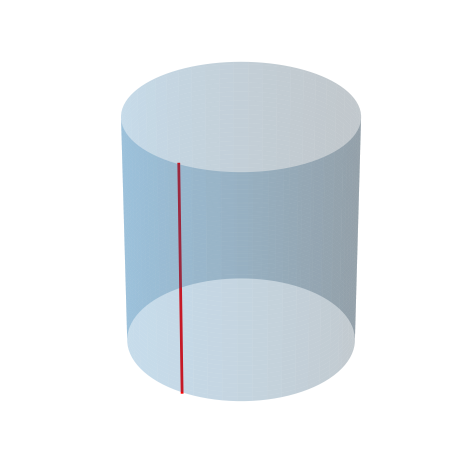
\includegraphics[width=0.9\textwidth]{images/cylinder_line.png}
 	  \caption{Vertical Line: case $b=0$}
	  \label{subfig:vertical}
	\end{subfigure}
	\hfill
	%------------------------------
	% Subfigure 2: Helix on the Cylinder
	\begin{subfigure}[b]{0.3\linewidth}
	  \centering
	  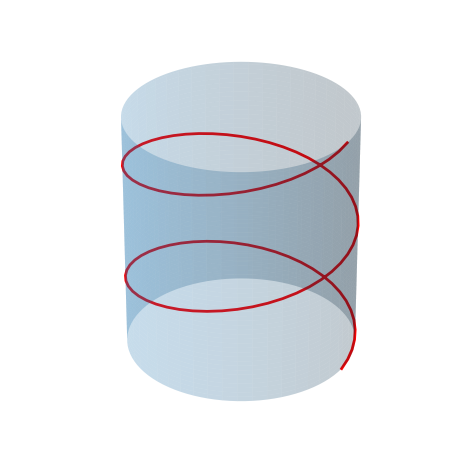
\includegraphics[width=0.9\textwidth]{images/cylinder_helix.png}
	  \caption{Helix: case $b\neq 0$}
	  \label{subfig:helix}
	\end{subfigure}
	\hfill
	%------------------------------
	% Subfigure 3: Horizontal Circle on the Cylinder
	\begin{subfigure}[b]{0.3\linewidth}
	  \centering
	  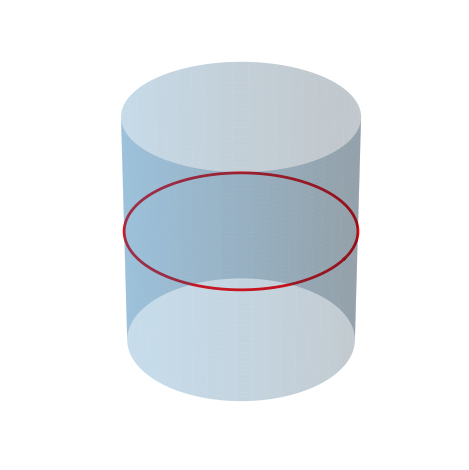
\includegraphics[width=0.9\textwidth]{images/cylinder_circle.png}
	  \caption{Circle: case $c=0$}
	  \label{subfig:circle}
	\end{subfigure}
	%------------------------------
	\caption{Geodesics on a Cylinder}
	\label{fig:geodesics-on-cylinder}
\end{figure}
  
\subsection{The Sphere}

We now consider the case of a sphere, which is a special case of a surface of revolution.
The sphere is a surface of revolution obtained by rotating a circle about an axis.
The parametric representation of the sphere is given by
\[
    \mathbf{r}(u, v) = \begin{bmatrix} R \cos (u) \cos (v) \\ R \cos (u) \sin (v) \\ R \sin (u) \end{bmatrix},
\]
where \(R\) is the radius of the sphere, \(u = \theta\) is the angle of rotation about the \(z\)-axis, and \(v = \phi\) is the angle of rotation about the \(x\)-axis.
The tangent vectors are given by
\[
    \mathbf{r}_u = \begin{bmatrix} -R \sin (u) \cos (v) \\ -R \sin (u) \sin (v) \\ R \cos (u) \end{bmatrix}, \quad \mathbf{r}_v = \begin{bmatrix} -R \cos (u) \sin (v) \\ R \cos (u) \cos (v) \\ 0 \end{bmatrix}.
\]
The metric for the sphere is given by
\[
    ds^2 = R^2 du^2 + R^2 \sin^2 (u) dv^2,
\]
Where the components of the metric tensor are given by \(E = R^2 \), \(F = 0\), and \(G = R^2 \sin^2 (u)\).
Thus the geodesic equations for the sphere are given by
\begin{align*}
    \ddot{u} + \sin(v) \cos(v) \dot{v}^2 &= 0 \\
    \ddot{v} + 2\tan(v) \dot{u} \dot{v} &= 0 
\end{align*}
The resulting system is a highly complex set of nonlinear differential equations, and in practice, geodesic equations are seldom solved directly.

This is where Clairaut's relation comes in handy.
We can use Clairaut's relation to simplify the geodesic equations.
We see that taking the derivatives of the metric tensor components with respect to \(v\) we have $E_v = 0$ and $G_v = 0$ which means that the sphere is a $u$-Clairaut parametrization.
Using Eq \eqref{eq:v_Clairaut_integral}, we get the following integral:
\[
    v = \pm \int \frac{c}{\sin(u)\sqrt{R^2\sin^{2}(u) - c^{2}}} \dd{u}
\]
We wont show the steps to solve this integral, as it is a bit tedious and not needed to understand the geodesic equations.
They can be found in full in \cite{oprea2007differential}, (Note: \cite{oprea2007differential} uses $v$-Clairaut parametrization, so the integration steps will slightly differ).
The solution to this integral is given by 
\[
\sin(v - d) = \lambda \cot(u)
\]
where \(d\) is a constant of integration and \(\lambda = \frac{c}{\sqrt{R^2 - c^2}}\).

Using the trigonometric identity \(\sin(v - d) = \sin(v)\cos(d) - \cos(v)\sin(d)\),  and find a common denominator $\sin(u)$ to get
\[
    \frac{\sin(v)\sin(u)}{\sin(u)}\cos(d) - \frac{\cos(v)\sin(u)}{\sin(u)}\sin(d) - \lambda \frac{\cos(u)}{\sin(u)} = 0
\]
If we substitute \(x = \cos(v)\sin(u), \quad y = \sin(v)\sin(u), \quad z = \cos(u)\), we can rewrite the equation as
\[
    y\cos(d) - x\sin(d) - \lambda z = 0
\]
Hence, the geodesic equations imply that the geodesics on the sphere lie on a plane \( ax + by + cz = d \) that passes through the origin.
So the geodesics on the sphere are great circles. Figure (\ref{fig:geodesics-on-sphere}) shows the geodesics on a sphere.

\begin{figure}[ht]
	\centering
	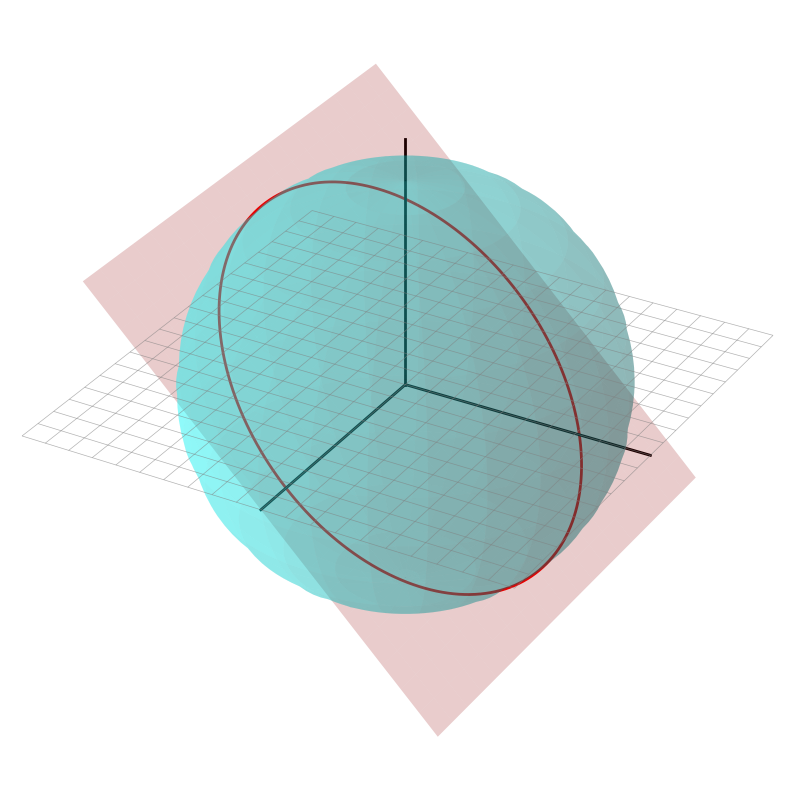
\includegraphics[width=0.4\textwidth]{images/output.png}
	\caption{Geodesics on a Sphere}
	\label{fig:geodesics-on-sphere}
\end{figure}

\subsection{The Hyperboloid}

Now we consider the case of a hyperboloid, which is a bit more complex to study than the sphere.
The hyperboloid is a surface of revolution obtained by rotating a hyperbola about an axis.
The parametric representation of the hyperboloid (also called a ”Hyperboloid of one sheet”) is given by
\[
    \mathbf{r}(u, v) = \begin{bmatrix} a \cosh (u) \cos (v) \\ a \cosh (u) \sin (v) \\ b \sinh (u) \end{bmatrix},
\]
where \(a\) and \(b\) are the semi-major and semi-minor axes of the hyperbola, respectively.

The tangent vectors are given by
\[
    \mathbf{r}_u = \begin{bmatrix} a \sinh (u) \cos (v) \\ a \sinh (u) \sin (v) \\ b \cosh (u) \end{bmatrix}, \quad \mathbf{r}_v = \begin{bmatrix} -a \cosh (u) \sin (v) \\ a \cosh (u) \cos (v) \\ 0 \end{bmatrix}.
\]
The metric for the hyperboloid is given by
\[
    ds^2 = ((a^2 + b^2)\sinh^{2}(u) + b^2) du^2 + a^2 \cosh^{2}(u) dv^2
\]
where \(E = (a^2 + b^2)\sinh^{2}(u) + b^2\), \(F = 0\), and \(G = a^2 \cosh^{2}(u)\).
Taking the derivatives of the components of the metric tensor, we find
\[
    E_u = 2(a^2 + b^2)\sinh(u)\cosh(u), \quad E_v = 0, \quad G_u = 2a^2 \sinh(u) \cosh(u), \quad G_v = 0.
\]
Thus, the hyperboloid is a $u$-Clairaut parametrization.
So the geodesic equations for the hyperboloid are given by
\begin{align*}
    \ddot{u} + \frac{(a^2 + b^2)\sinh(u)\cosh(u)}{(a^2 + b^2)\sinh^{2}(u) + b^2}\,\dot{u}^2 - \frac{a^2 \sinh(u) \cosh(u)}{(a^2 + b^2)\sinh^{2}(u) + b^2}\,\dot{v}^{2} &= 0 \\
    \ddot{v} + \tanh(u) \dot{u} \dot{v} &= 0
\end{align*}
Using Clairaut's relation, we can simplify the geodesic equations.
Since $E_v = 0$ and $G_v = 0$, we have a $u$-Clairaut parametrization for the hyperboloid.
Using Eq \eqref{eq:v_Clairaut_integral}, we get
\[
    v = \pm \int \frac{c\sqrt{(a^2 + b^2)\sinh^2(u) + b^2}}{a\cosh(u)\sqrt{a^2\cosh^2(u) - c^2}}\,\dd{u}
\]
Obviously, this integral is not trivial to solve, but we can use Clairaut's relation to analyze the geodesics on the hyperboloid.
We have that Clairaut's relation for the hyperboloid is given by
\[
    a \cosh(u) \sin(\phi) = C  
\]
As shown in \cite{khuangsatung2012geodesics}, by assuming that $u$ is very small number, we can consider the following cases:
\begin{itemize}
    \item If $C = 0$, then $\phi = 0$ and the geodesic corresponds to a meridian on the hyperboloid.
    \item If $C = a$ at $u = u_0 = 0$, then $\phi = \frac{\pi}{2}$ and the geodesic a parallel on the hyperboloid.
    \item If $\abs{C} < \abs{a}$, then $\phi$ is a constant angle and the geodesic is a helix on the hyperboloid.
\end{itemize}


\begin{figure}[ht]
	\centering
	%------------------------------
	% Subfigure 1: Vertical Line on the Cylinder
	\begin{subfigure}[b]{0.4\linewidth}
	  \centering
	  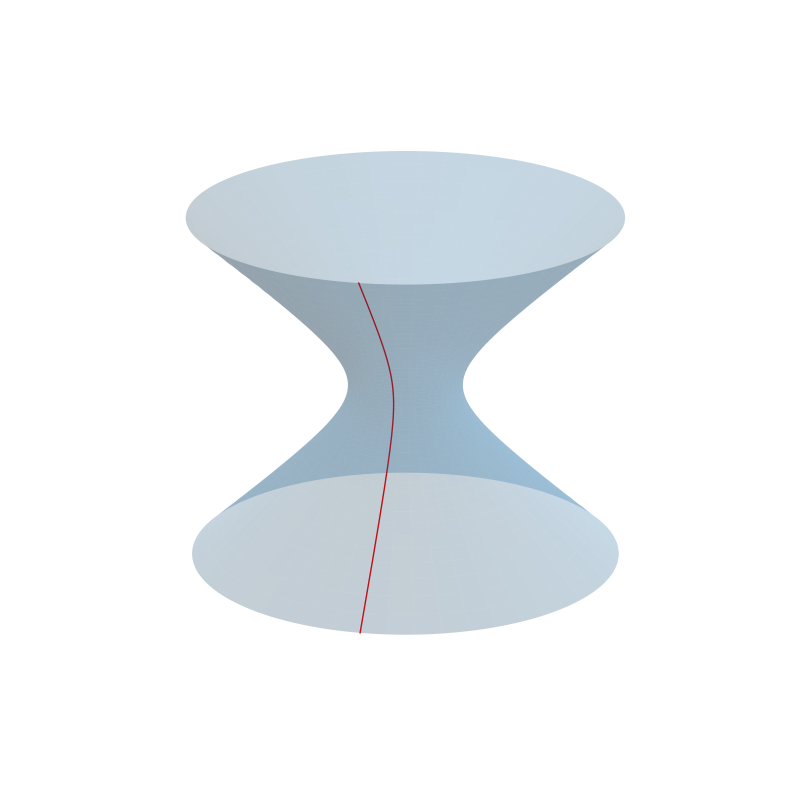
\includegraphics[width=1.0\textwidth]{images/h_merd1.png}
 	  \caption{Meridian: case $C=0$}
	  \label{subfig:vertical}
	\end{subfigure}
	\hfill
	%------------------------------
	% Subfigure 2: Helix on the Cylinder
	\begin{subfigure}[b]{0.4\linewidth}
	  \centering
	  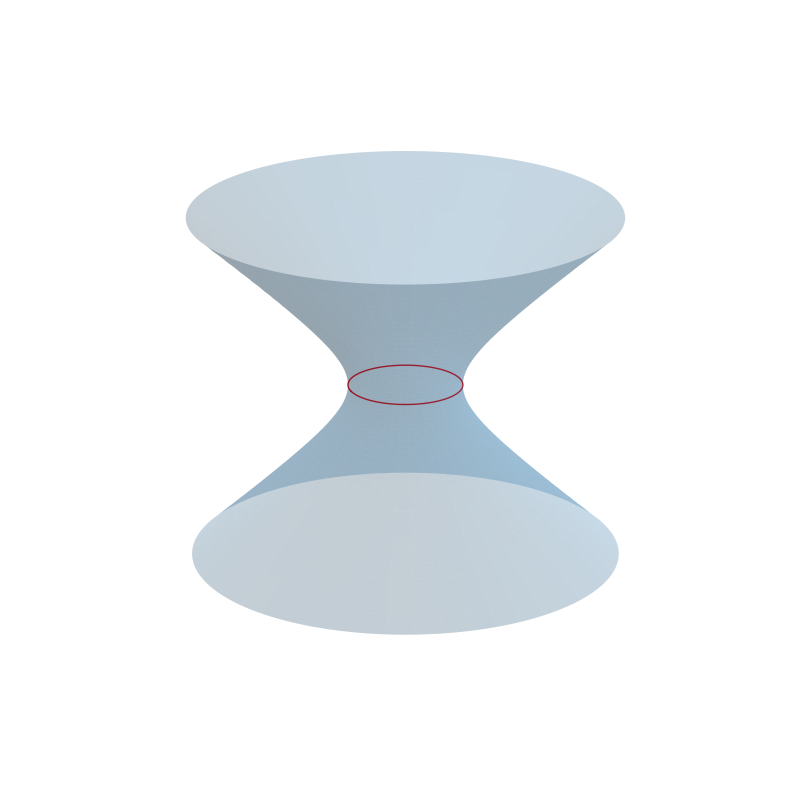
\includegraphics[width=1.0\textwidth]{images/h_circ1.png}
	  \caption{Parallel: case $C=a$}
	  \label{subfig:helix}
	\end{subfigure}
	\hfill
	%------------------------------
	% Subfigure 3: Horizontal Circle on the Cylinder
	\begin{subfigure}[b]{0.4\linewidth}
	  \centering
	  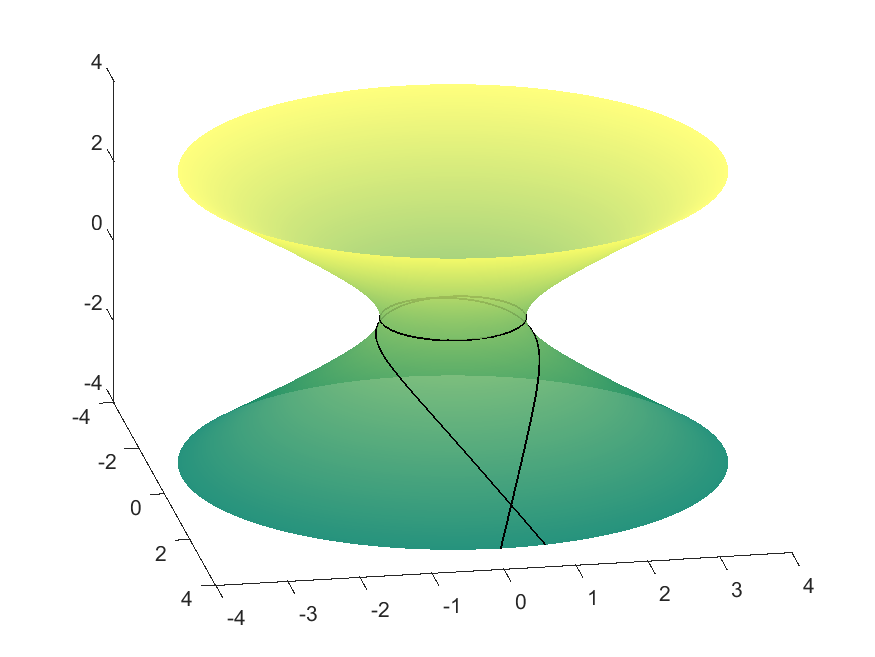
\includegraphics[width=1.0\textwidth]{images/hyperboloid1.png}
	  \caption{Helical case $C \neq 0$}
	  \label{subfig:circle}
	\end{subfigure}
	%------------------------------
	\caption{Geodesics on a Cylinder}
	\label{fig:geodesics-on-cylinder}
\end{figure}

\subsection{The Torus}

The torus is a surface of revolution obtained by rotating a circle about an axis that is not in the plane of the circle.
The parametric representation of the torus is given by
\[
    \mathbf{r}(u, v) = \begin{bmatrix} (R + r \cos (u)) \cos (v) \\ (R + r \cos (u)) \sin (v) \\ r \sin (u) \end{bmatrix},
\]
where \(R\) is the distance from the center of the torus to the center of the tube, and \(r\) is the radius of the tube.
The tangent vectors are given by
\[
    \mathbf{r}_u = \begin{bmatrix} -r \sin (u) \cos (v) \\ -r \sin (u) \sin (v) \\ r \cos (u) \end{bmatrix}, \quad \mathbf{r}_v = \begin{bmatrix} -(R + r \cos (u)) \sin (v) \\ (R + r \cos (u)) \cos (v) \\ 0 \end{bmatrix}.
\]
The metric for the torus is given by
\[
    ds^2 = r^2 du^2 + (R + r \cos (u))^2 dv^2,
\]
where \(E = r^2\), \(F = 0\), and \(G = (R + r \cos (u))^2\).
Taking the derivatives of the components of the metric tensor, we find
\[
    E_u = 0, \quad E_v = 0, \quad G_u = -2(R + r \cos (u))r \sin (u), \quad G_v = 0.
\]

It follows that the only nonzero Christoffel symbols are
\[
  \Gamma^u_{vv}
    =-\frac{G_u}{2E}
    =\frac{(R+r\cos u)\sin u}{r},
  \qquad
  \Gamma^v_{uv}
    =\Gamma^v_{vu}
    =\frac{G_u}{2G}
    =-\frac{r\sin u}{R+r\cos u}.
\]
Accordingly, the geodesic equations (with respect to arc length \(s\)) become
\begin{align*}
  \ddot u + \frac{(R+r\cos u)\sin u}{r}\,\dot v^2 &= 0,\\
  \ddot v - \frac{2r\sin u}{R+r\cos u}\,\dot u\,\dot v &= 0,
\end{align*}

Using Clairaut's relation, we can simplify the geodesic equations.
Using Eq \eqref{eq:v_Clairaut_integral}, we get
\[
  v = v_0\pm\int \frac{C\,r}{(R+r\cos u)\,\sqrt{(R+r\cos u)^2 - C^2}} \,du.
\]
We can use Clairaut's relation to analyze the geodesics on the torus.
\[
    (R + r \cos (u)) \sin(\phi) = C
\]
By assuming that $u$ is very small number, therefore we will consider into 3 cases:

\begin{itemize}
  \item \(C=0\).  Then \(\sin\phi=0\), so \(\dot v=0\):  these are the meridians \(v=\mathrm{const}\).
  \item \(\lvert C\rvert=R+r\) (attained at \(u=0\)).  Then \(\sin\phi=1\):  the outer parallel \(u=0\).
  \item \(\lvert C\rvert=\lvert R-r\rvert\) (attained at \(u=\pi\)).  Then \(\sin\phi=1\):  the inner parallel \(u=\pi\).
  \item \(0<\lvert C\rvert<R-r\).  Geodesics wind unboundedly, crossing both the inner and outer parallels.
  \item \(R-r<\lvert C\rvert<R+r\).  Geodesics oscillate between the two “barrier” parallels given by \(R+r\cos u=\pm C\).
\end{itemize}

\begin{figure}[ht]
	\centering
	%------------------------------
	% Subfigure 1: Vertical Line on the Cylinder
	\begin{subfigure}[b]{0.4\linewidth}
	  \centering
	  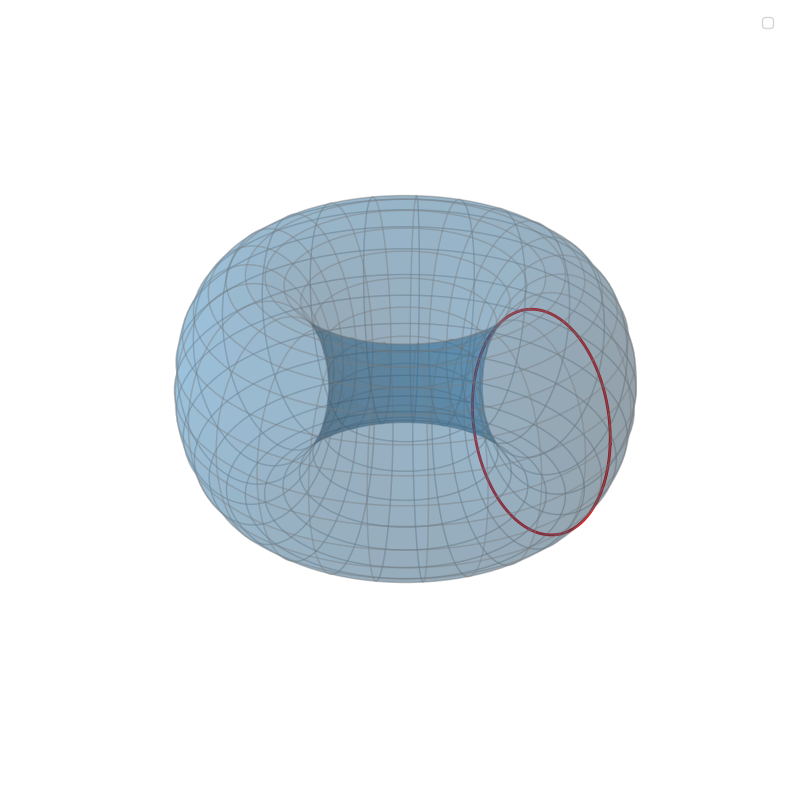
\includegraphics[width=1.0\textwidth]{images/torus_merd.png}
 	  \caption{Meridian: case $C=0$}
	  \label{subfig:vertical}
	\end{subfigure}
	\hfill
	%------------------------------
	% Subfigure 2: Helix on the Cylinder
	\begin{subfigure}[b]{0.4\linewidth}
	  \centering
	  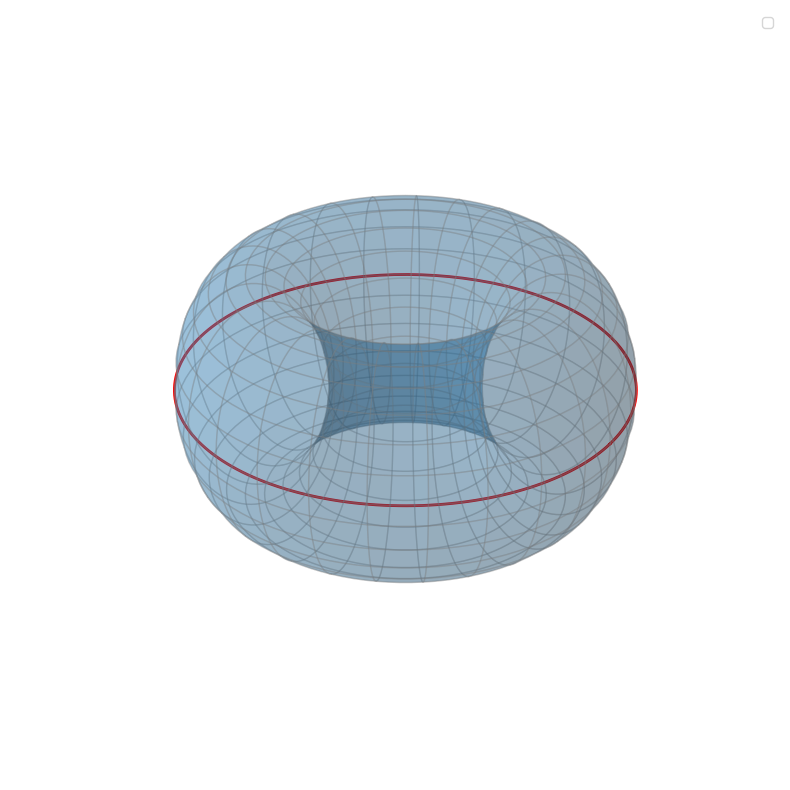
\includegraphics[width=1.0\textwidth]{images/torus_par.png}
	  \caption{Parallel: case $C=R+r$}
	  \label{subfig:helix}
	\end{subfigure}
	\hfill
	%------------------------------
	% Subfigure 3: Horizontal Circle on the Cylinder
	\begin{subfigure}[b]{0.4\linewidth}
	  \centering
	  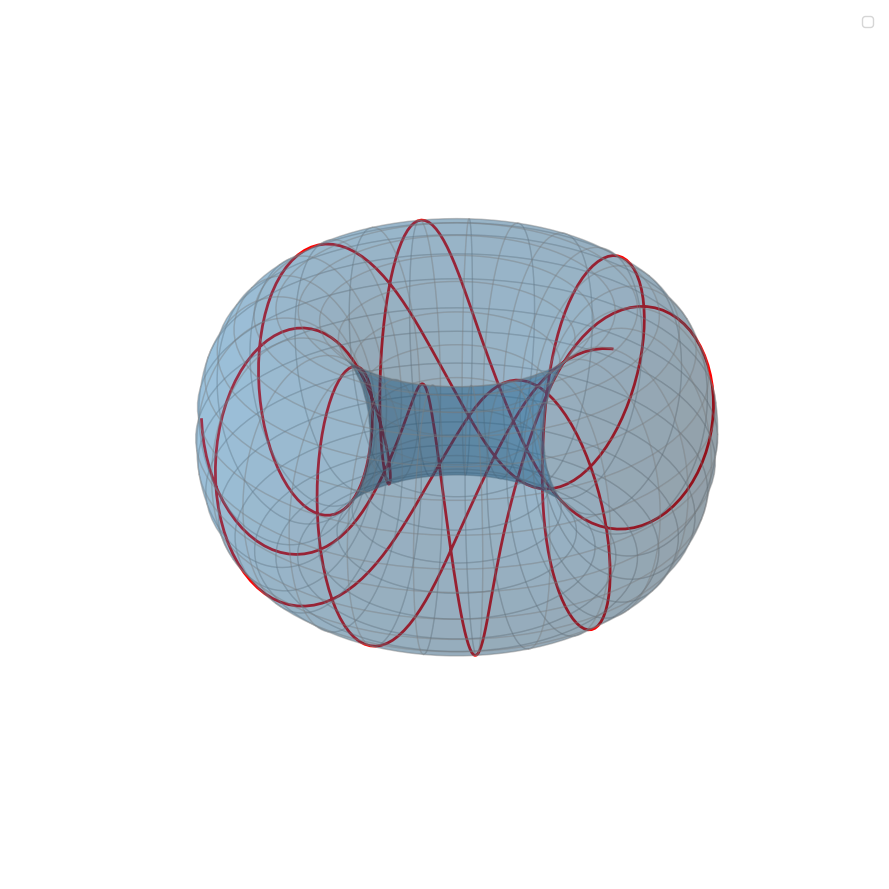
\includegraphics[width=1.0\textwidth]{images/torus_ub1.png}
	  \caption{Unbounded: case $C \in (0, R-r)$}
	  \label{subfig:circle}
	\end{subfigure}
	%------------------------------
	\caption{Geodesics on a Cylinder}
	\label{fig:geodesics-on-cylinder}
\end{figure}

\section{Symmetries, Isometries, and Killing Vector Fields}

To be able to simplify the process of finding geodesics, we can leverage the existing symmetries inherent to a manifold.
In this section, we review the algebraic framework of continuous symmetries—embodied in the notion of a group—and then explain how these symmetries manifest as isometries through the use of Killing vector fields. 

Symmetries are transformations that leave the geometric structure of an object unchanged.
For example, consider a square. The symmetries of the square include rotations by \(0^\circ\), \(90^\circ\), \(180^\circ\), and \(270^\circ\), as well as reflections across its diagonals and midlines.
These transformations can be combined in various ways, such as performing a rotation followed by a reflection.

\subsection{Groups and Continuous Symmetries}
When working with a set of symmetries, it is often useful to organize them into a mathematical structure called a \emph{group}.
Informally, a group is a collection of operations (such as rotations, translations, or reflections) that can be combined (via composition) while preserving the object's essential properties. 
More formally, we recall the following definition.

\begin{definition}[Group]
	A set $G$ equipped with a binary operation $\circ: G \times G \to G$ is called a \emph{group} if the following properties hold:
	\begin{enumerate}
	    \item (\textbf{Closure}) For all $a,b \in G$, the product $a \circ b$ is also in $G$.
	    \item (\textbf{Associativity}) For all $a,b,c \in G$, $(a \circ b) \circ c = a \circ (b \circ c)$.
	    \item (\textbf{Identity}) There exists an element $e \in G$ such that $e \circ a = a \circ e = a$ for every $a \in G$.
	    \item (\textbf{Inverses}) For every $a \in G$, there exists an element $a^{-1} \in G$ satisfying $a \circ a^{-1} = a^{-1} \circ a = e$.
	\end{enumerate}
\end{definition}

A interesting group is the \emph{Lie group}, which is a group that is also a smooth manifold.
This means that the topological structure of the group is compatible with the smooth structure of the manifold.
An example of a Lie group is the group of rotations in $n$-dimensional space, denoted by $SO(n)$ called the \emph{Special Orthogonal group}.
The elements of this group are orthogonal matrices with determinant 1, and the group operation is matrix multiplication.
The Special Orthogonal group $SO(n)$ is isomorphic (i.e., structurally identical) to the $n-1$-dimensional sphere $S^{n-1}$.
This is helpful when describing the symmetries of a manifold such as surfaces of revolution.
Lie groups are important in physics and mathematics because they provide a framework for understanding continuous symmetries.

Let us look at the group of symmetries associated with the surfaces of revolution we have seen so far.
\begin{itemize}
	\item \textbf{Cylinder:} Since the cylinder is topologically given by $S^1 \times \mathbb{R}$, the symmetry group is the direct product of the circle group $SO(2)$ and the translation group $\mathbb{R}$, which corresponds to the rotations about the $z$-axis and translations along the $z$-axis.
	\item \textbf{Sphere:} Because the sphere is topologically given by $S^2$, the symmetry group is the rotation group $SO(3)$, which corresponds to the rotations about any axis in three-dimensional space.
	\item \textbf{Hyperboloid:} Since hyperboloids describe Minkowski spacetime (which models the universe), the symmetry group is the Lorentz group $SO(1,2)$, which corresponds to the rotations and boosts in Minkowski spacetime.
	\item \textbf{Torus:} The torus is topologically given by $S^1 \times S^1$, and the symmetry group is the direct product of two circle groups $SO(2) \times SO(2)$, which corresponds to the rotations about the $z$-axis and the rotation about the $x$-axis.
\end{itemize}

A manifold, such as a surface $\mathcal{S}$, possesses a symmetry if there exists a diffeomorphism $\phi: \mathcal{S} \to \mathcal{S}$ from the manifold to itself that preserves the geometric structure.
This means that the metric tensor $g$ remains invariant under the transformation:
\[
	\phi \circ g = g,
\]
The set of all such diffeomorphisms forms a group, called the \emph{symmetry group} of the manifold.

\subsection{Isometries on Surfaces}
Now we look at specific types of symmetries that preserve the metric structure of a surface called \emph{isometries}.
Given a surface $\mathcal{S}$ with a metric $g$, an \emph{isometry} is a transformation that preserves distances. More precisely, a bijective map
\[
f: S \to S
\]
is an \emph{isometry} if, for all points $p,q\in S$, the distance between $p$ and $q$ equals the distance between their images:
\[
d\big(f(p),f(q)\big)=d(p,q).
\]
This invariance implies that the local expressions for the metric coefficients remain unchanged under the transformation. 
One thing to note is that all isometries are symmetries, but not all symmetries are isometries.
For example, consider the rotation of a circle about its center. This transformation preserves the distances between points on the circle, and thus it is an isometry.
However, a shear transformation that distorts the circle into an ellipse does not preserve distances and is not an isometry.

\subsection{Killing Vector Fields}
A Killing vector field (named after the mathematician Wilhelm Killing) is a vector field on a manifold that generates an isometry of the metric.

\begin{definition}[Killing Vector Field]
	Let \(M\) be a manifold with metric \(g\). A vector field \(K\) on \(M\) is called a \emph{Killing vector field} if the Lie derivative of the metric with respect to \(K\) vanishes:
	\[
		\mathcal{L}_{K} (g) = 0.
	\]
	This means that the flow generated by \(K\) preserves the metric, and hence the distances and angles on the manifold.
\end{definition}
The Lie derivative of the metric with respect to a vector field \(K\) is given by
\[
	\mathcal{L}_{K} (g_{\mu\nu}) = \nabla_{\mu} K^{\mu} + \nabla_{\nu} K^{\nu},
\]
Where \(\nabla\) is the covariant derivative associated with the metric \(g\).
We wont go into details of what the Lie derivative is, but it is a way to measure how a tensor field changes along the flow of a vector field.
For more details, see \cite{oprea2007differential},\cite{note32020covariant},\cite{atkins2018solving},\cite{carrol2019spacetime}.

For the purposes of this thesis, we not be using the Lie derivative definition to find the Killing vector field, but rather we will be finding them by looking for the coordintates of which the metric is independent off.

As shown in \cite{carrol2019spacetime} and \cite{atkins2018solving}, if $K^{\mu}$ is a Killing vector field, then we have the following to holds
\begin{equation}\label{eq:Killing_vector}
	\text{const} = g_{\mu\nu}K^{\mu}\dv{x^{\nu}}{\lambda} 
\end{equation}

Additionally, we have another constant for the motion along the geodesic, which is given by
\begin{equation}\label{eq:epsilon_equation}
	\epsilon = - \sum_{\mu,\nu} g_{\mu\nu}\dv{x^{\mu}}{\lambda}\dv{x^{\nu}}{\lambda}
\end{equation}
In the context of general relativity, this equation describes the motion of a test particle in a gravitational field where \(\epsilon = 0\) for null geodesics, \(\epsilon = 1\) for time-like geodesics, and \(\epsilon = -1\) for space-like geodesics.

\subsection{Clairaut's Relation from Killing Vector Fields}

We now will show how to derive Clairaut's relation from the conservation law associated with a Killing vector field.
Consider a surface of revolution obtained by rotating a profile curve around an axis, with local coordinates $(u,v)$ so that the induced metric reads
$$
ds^2 \;=\; du^2 \;+\; f(u)^2\,dv^2\,,
$$
where $f(u)$ is the distance from the axis.

Because the metric coefficients do not depend on $v$, the angular coordinate, we thus have that rotations about the axis are isometries of the metric.
We then have the following Killing vector field:
\begin{align*}
	K^{2} &= \begin{bmatrix} 0 \\ 1 \end{bmatrix} \\
\end{align*}

Using equation \eqref{eq:Killing_vector}, we find the following conserved quantity $L$ along the geodesic:
\begin{align*}
	L &= g_{22} K^{2} \dv{x^{2}}{s} \\
	&= f(u)^2 \dv{v}{s} \\
	&= \text{const}
\end{align*}

Going back to the unit speed condition for a curve in a surface of revolution, we have
\begin{align*}
	1 &= \left(\dv{u}{s}\right)^2 + f(u)^2 \left(\dv{v}{s}\right)^2 \\
\end{align*}

Using the trigonometric identity \( \sin^2(\phi) + \cos^2(\phi) = 1 \), we can rewrite the unit speed condition as
\[
	\sin^2(\phi) + \cos^2(\phi) = \left(\dv{u}{s}\right)^2 + f(u)^2 \left(\dv{v}{s}\right)^2
\]
Where we have
\[
	\cos(\phi) = \dv{u}{s} \qquad \sin(\phi) = f(u)\dv{v}{s}
\]

We can thus clearly see that the constant \(L\) is given by
\[
	L = f(u) \sin(\phi)
\]
Thus we have derived Clairaut's relation from the conservation law associated with the Killing vector field.

One can show that from just using equation \eqref{eq:Killing_vector} we can find the geodesics of a surface without the need of the geodesics equations.
Due to the inherent symmetries of the surface, we can find the geodesics by looking for the coordinates of which the metric is independent off and finding the Killing vector field associated with that symmetry.
Then we can use the conservation law associated with the Killing vector field to find the geodesics.
This is a powerful technique that can be used to find the geodesics of a surface without the need to solve the geodesic equations directly.


\subsection{Noether's Theorem}
We will connect the conserved quantities associated with the Killing vector fields to Noether's theorem.
In the context of classical mechanics, Noether's theorem provides a profound connection between symmetries and conservation laws.
\begin{theorem}[Noether's Theorem]
	For every continuous symmetry in a physical system, there exists a conservation law.
	So given a diffeomorphism \( \phi: M \to M \) that leaves the action invariant, there exists a conserved quantity associated with the symmetry.
\end{theorem}
For instance, consider the following standard symmetries:
\begin{itemize}
    \item Invariance under time translations implies conservation of energy.
    \item Invariance under spatial translations implies conservation of linear momentum.
    \item Invariance under rotations implies conservation of angular momentum.
\end{itemize}
We see that when studying physical systems, we can use Noether's theorem to find conserved quantities associated with symmetries.
In the context of general relativity, we can use Noether's theorem to find conserved quantities associated with the symmetries of the spacetime geometry.
In particular, we can use Noether's theorem to find the conserved quantities associated with the Killing vector fields of the spacetime geometry.

\section{A look to Black Holes Geodesics}

In this section, we will look at the geodesics of a black hole.
We will use the Schwarzschild metric, which describes the spacetime geometry outside a spherically symmetric, non-rotating mass. The Schwarzschild metric is given by
\begin{equation}\label{eq:schwarzschild_metric}
	ds^2 = -\left(1 - \frac{2GM}{r}\right) dt^2 + \left(1 - \frac{2GM}{r}\right)^{-1} dr^2 + r^2 d\Omega^2
\end{equation}
where 
\[
d\Omega^2 = d\theta^2 + \sin^2(\theta) d\phi^2
\] 
is the metric on the unit sphere, \(G\) is the gravitational constant, \(M\) is the mass of the black hole, and \(c = 1\) is the speed of light under natural units.
The Schwarzschild metric is a solution to the Einstein field equations in general relativity and describes the spacetime geometry around a non-rotating, spherically symmetric black hole.
The metric describes the $4$-dimensional spacetime geometry, where \(t\) is the time coordinate, \(r\) is the radial coordinate, \(\theta\) is the polar angle, and \(\phi\) is the azimuthal angle.

Because the Schwarzschild metric is a spherically symmetric solution, we can choose to study the geodesics in the equatorial plane, where \(\theta = \frac{\pi}{2}\), since regardless of the value of \(\theta\), the geodesics will be the same due to the rotational symmetry of the spacetime.
This means that we can set \(\theta = \frac{\pi}{2}\) and \(d\theta = 0\) in the metric.
This simplifies the metric to
\begin{equation}\label{eq:schwarzschild_metric_equatorial}
	ds^2 = -\left(1 - \frac{2GM}{r}\right) dt^2 + \left(1 - \frac{2GM}{r}\right)^{-1} dr^2 + r^2 d\phi^2
\end{equation}
This in turn converts our metric from a 4D metric to a 3D metric, for which we can use to visualize the geodesics in 2D.
The metric tensor is given by
\[
	g_{\mu\nu} = \begin{bmatrix}
	-\left(1 - \frac{2GM}{r}\right) & 0 & 0 \\
	0 & \left(1 - \frac{2GM}{r}\right)^{-1} & 0 \\
	0 & 0 & r^2
	\end{bmatrix}
\]
Because the metric is independent of the coordinates \(t\) and \(\phi\), we can use the Killing vector fields associated with these symmetries to find conserved quantities along the geodesics.
The Killing vector fields associated with the Schwarzschild metric are given by
\begin{align*}
	\xi^{1} &= \frac{\partial}{\partial t} = \begin{bmatrix} 1 \\ 0 \\ 0 \end{bmatrix} \\
	\xi^{3} &= \frac{\partial}{\partial \phi} = \begin{bmatrix} 0 \\ 0 \\ 1 \end{bmatrix}
\end{align*}
The conserved quantities associated with these Killing vector fields are given by
\begin{align}
	E &= -g_{11} \, \xi^{1} \, \dv{x^{1}}{\lambda} = \left(1 - \frac{2GM}{r}\right) \dv{t}{\lambda} \label{eq:energy} \\
	L &= g_{33} \, \xi^{3} \, \dv{x^{3}}{\lambda} = r^2 \dv{\phi}{\lambda} \label{eq:angular_momentum}
\end{align}
where \(E\) is the energy of the particle and \(L\) is the angular momentum of the particle.

Pluggin this into Eq.(\ref{eq:epsilon_equation}), we get
\begin{align*}
	\epsilon &= -g_{\mu\nu}\dv{x^{\mu}}{t}\dv{x^{\nu}}{t} = -g_{tt} \left(\dv{t}{\lambda}\right)^2 - g_{rr} \left(\dv{r}{\lambda}\right)^2 - g_{\phi\phi} \left(\dv{\phi}{\lambda}\right)^2 \\
	&= -\left(1 - \frac{2GM}{r}\right) \left(\dv{t}{\lambda}\right)^2 - \left(1 - \frac{2GM}{r}\right)^{-1} \left(\dv{r}{\lambda}\right)^2 - r^2 \left(\dv{\phi}{\lambda}\right)^2
\end{align*}

Moving $\epsilon$ to the other side, and multiplying by $g_{tt}$, we get
\[
	0 = \left(1 - \frac{2GM}{r}\right)^{2} \left(\dv{t}{\lambda}\right)^2 + \left(\dv{r}{\lambda}\right)^2 + \left(1 - \frac{2GM}{r}\right) \left(r^2 \left(\dv{\phi}{\lambda}\right)^2 + \epsilon \right)
\]
Substituting the expressions for \(E\) and \(L\) from Eq.(\ref{eq:energy}) and Eq.(\ref{eq:angular_momentum}), we get
\begin{equation}
	0 = -E^{2} + \left(\dv{r}{\lambda}\right)^2 + \left(1 - \frac{2GM}{r}\right) \left(\frac{L^{2}}{r^{2}} + \epsilon \right)
\end{equation}

Expanding the last term and dividing by $2$, we get
\[
	\frac{1}{2} \left(\dv{r}{\lambda}\right)^2 + \frac{1}{2} \left(1 - \frac{2GM}{r}\right) \left(\frac{L^{2}}{r^{2}} + \epsilon \right) = \frac{E^{2}}{2}
\]
This is the effective potential for the Schwarzschild metric, and it describes the motion of a particle in the gravitational field of a black hole.
The effective potential is given by
\begin{equation}
	V_{\text{eff}}(r) = \left(1 - \frac{2GM}{r}\right) \left(\frac{L^{2}}{r^{2}} + \epsilon \right) = \epsilon - \epsilon\frac{2GM}{r} + \frac{L^{2}}{r^{2}} - \frac{2GM L^{2}}{r^{3}}
\end{equation}
The effective potential describes the motion of a particle in the gravitational field of a black hole, and it can be used to analyze the stability of orbits around the black hole.

\subsection{Schwarzschild Radius}
For a black hole, with some mass \(M\), its event horizon (i.e. the surface beyond which nothing can escape) is located at the Schwarzschild radius, which is given by
\[
	r_{s} = \frac{2GM}{c^{2}} = 2GM
\]
with \(c = 1\) in natural units.
The Schwarzschild radius is the radius of the event horizon of a black hole, and it is the point at which the gravitational pull of the black hole becomes so strong that nothing, not even light, can escape from it.
\subsection{Circular Orbits}
Circular orbits are a special case of geodesics in the Schwarzschild metric, where the radial coordinate \(r\) is constant.
We find a circular orbit at $r = r_{c}$ that satisfies the following:
\[
	\dv{V_{\text{eff}}}{r}\Bigg|_{r_{c}} = 0
\]
Taking the derivative of the effective potential, we get
\begin{equation}\label{eq:dV_eff}
	\dv{V_{\text{eff}}}{r}\Bigg|_{r_{c}} = \frac{2GM\epsilon}{r_{c}^{2}} - \frac{2L^{2}}{r_{c}^{3}} + \frac{6GM L^{2}}{r_{c}^{4}}
\end{equation}
Multiplying by $r_{c}^{4}/2$, we get
\[
	0 = GM\epsilon r_{c}^{2} - L^{2} r_{c} + 3GM L^{2}
\]

\subsection{Null Geodesics}

In Newtonian gravity, only massive objects feel the gravitational attraction of other masses, so massless particles like photons travel along straight lines in a flat spacetime described by the Minkowski metric \cite{carrol2019spacetime}.  
By contrast, in general relativity gravity is encoded as curvature of spacetime around a mass, and light rays follow this curvature.  
Because photons trajectories are not affected by the mass of the object they are passing by, and thus must follow straight lines in the curved spacetime, we can use the geodesic equations to describe their motion.
These light-ray trajectories are called \emph{null geodesics}, characterized by \ref{eq:epsilon_equation} with \(\epsilon = 0\).

For circular null orbits in the Schwarzschild metric, we set \(\epsilon=0\) in equation \ref{eq:dV_eff} gives
\[
0 \;=\; -\,L^{2}\,r_{c} \;+\; 3\,G\,M\,L^{2},
\]
where \(L\) is the photon's conserved angular momentum per unit energy.  
Solving for \(r_{c}\) yields
\[
r_{c} \;=\; 3\,G\,M.
\]
This special radius \(r_{c}\) defines the \emph{photon sphere}—the locus where light can orbit the black hole in an unstable circular path. 
Any small radial perturbation will cause the photon to either spiral inward into the black hole or escape back to infinity.

We see that the photon sphere is located relatively close to the event horizon of the black hole, seperated by a factor of \(GM\).


\subsection{Time-like Geodesics}
For time-like geodesics, we have \(\epsilon = 1\), so we can rewrite the equation as
\[
	0 = GM r_{c}^{2} - L^{2} r_{c} + 3GM L^{2}
\]
This is a quadratic equation in \(r_{c}\), and we can use the quadratic formula to find the radius of the circular orbit:
\[
	r_{c} = \frac{L^{2} \pm \sqrt{L^{4} - 12GM L^{2}}}{2GM}
\]
This gives us two solutions for the radius of the circular orbit, one of which is stable and the other is unstable.
The stable solution is given by
\[
	r_{c} = \frac{L^{2} + \sqrt{L^{4} - 12GM L^{2}}}{2GM}
\]
The unstable solution is given by
\[
	r_{c} = \frac{L^{2} - \sqrt{L^{4} - 12GM L^{2}}}{2GM}
\]
The stable solution corresponds to a circular orbit that is stable under small perturbations, while the unstable solution corresponds to a circular orbit that is unstable under small perturbations.

\begin{figure}
	\centering
	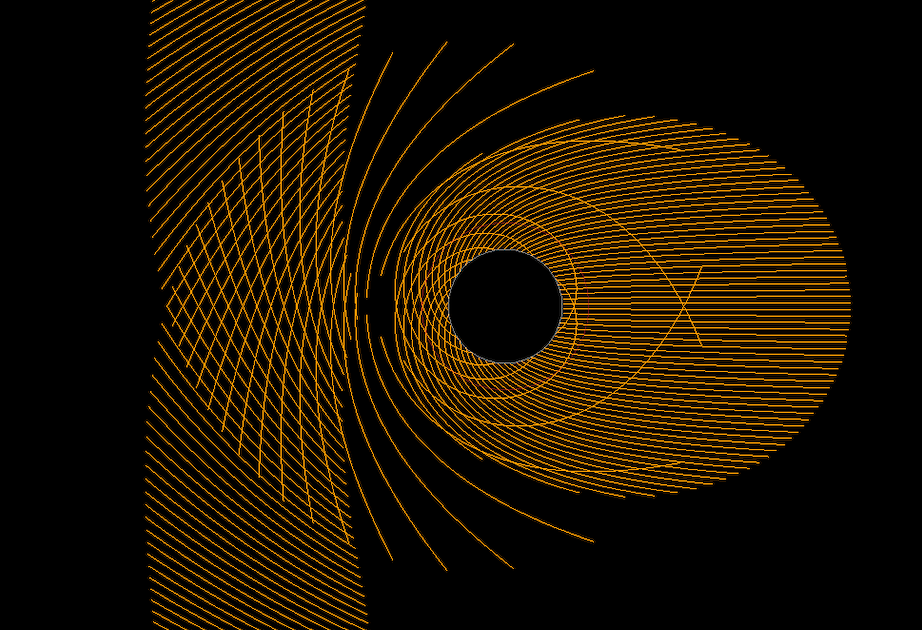
\includegraphics[width=0.5\textwidth]{images/bh_geo.png}
	\caption{Geodesics in the Schwarzschild metric.}
	\label{fig:bh_geo}
\end{figure}

% \color{black}
\section{Conclusion}

We have shown that a symmetry-centered approach unifies the study of geodesics across classical and relativistic settings.  
By deriving conserved quantities from Killing vector fields, one bypasses the full geodesic equations and reduces the problem to solving first-order integrals.  
On surfaces of revolution, this yields Clairaut’s relation and a clear classification of meridians, parallels, helices, and oscillatory trajectories. 
In the Schwarzschild spacetime, the same machinery produces the effective potential, circular orbits, and the photon sphere in a few lines.

\medskip\noindent\textbf{Future work.}  
The \emph{fundamental group} \(\pi_{1}(M)\) is the set of all loops in \(M\) based at a point \(x_{0}\), where two loops are considered the same if one can be continuously deformed into the other.  
We multiply two classes \([\gamma_{1}]\) and \([\gamma_{2}]\) by tracing \(\gamma_{1}\) then \(\gamma_{2}\).  

Comparing \(\pi_{1}(M)\) with the isometry group can tell us which loop-classes admit closed geodesics and how the surface’s symmetries affect their shape and stability.

\nocite{*}
\bibliographystyle{unsrt}
\bibliography{references}


\end{document}